\section{Methodology}
After having introduced the main concepts needed to understand the purpose of this work, it is possible now to enter the specifics of the work carried out. In this section, the specific pairs-trading strategy will be outlined, together with the benchmark pairs trading strategy used as comparison and the two factor models used to understand its PnL drivers.
\subsection{Strategy description}
The strategy selected to be analyzed has been the one introduced by \cite{ioannis_2023}. In their paper they outline a statistical arbitrage pairs trading strategy based on a two agent framework. 

One agent, the investor, has a cointegration model that indicates when in a pair one of the assets is relatively overvalued and the other is relatively undervalued. These mispricings are mean reverting, and the investor can profit from them by shorting the overvalued asset and buying the undervalued one. The other agent, the counter-party, receives the order flow from the investor taking the opposing position and is required by  operational mandate to continuously hedge the position and neutralize the portfolio. Within this framework, by maximizing the expected utility of the portfolio, the optimal weights for the investor are shown to be the deltas of a spread option on the two assets. 

The basic cointegration model used by the investor of two assets with prices $y_t$ and $x_t$ is 
\begin{equation}
    \frac{dy_t}{y_t}=\mu_ydt-\lambda_1z_tdt+\sigma_ydW_{y,t}
\end{equation}
\begin{equation}
    \frac{dx_t}{x_t}=\mu_xdt+\lambda_2z_tdt+\sigma_xdW_{x,t}
\end{equation}
\begin{equation}
    z_t=\ln y_t - \ln x_t
\end{equation}

where $\mu_y$, $\mu_x$, $\lambda_1$, $\lambda_2$, $\sigma_y$ and $\sigma_x$ are constant parameters and $W_{y,t}$ and $W_{x,t}$ are standard Brownian motions with zero drift rate and unit variance rate. Additionally, the investor has a cash account $B_t$
with a constant return $r$ following the dynamics
\begin{equation}
    dB_t=rB_tdt
\end{equation}
With that, the investor's portfolio is the following.
\begin{equation}
    \label{e:portfolio-equation}
    \Pi_t=\delta_1 y_t + \delta_2 x_t + \delta_3 B_t
\end{equation}
Where $\delta_1$, $\delta_2$ and $\delta_3$ are the position sizes for the two assets and the cash account respectively. This portfolio equation is subject to the constraint 
\begin{equation}
    \delta_1 + \delta_2 + \delta_3 = 1
\end{equation}
ensuring the portfolio position is self financed between the long, short and cash positions. 

Having the two cointegrated assets, a call option written on the spread $y_t - x_t$ with payoff $\psi(y_T, x_T)=max(y_T-x_T,0)$ can be defined as 
\begin{equation}
    C(y_t,x_t,t)=y_t \Phi(d_1)-x_t \Phi(d_2)
    \label{spread_option}
\end{equation}
where:
\begin{equation}
    \label{e:calc-d1}
    d_1=\frac{\ln\left(\frac{y_t}{x_t}\right)+\frac{1}{2}\sigma^2_z(T-t)}{\sigma_z \sqrt{T-t}}
\end{equation}
\begin{equation}
    d_2=d_1-\sigma_z \sqrt{T-t}
\end{equation}
\begin{equation}
    \sigma_z=\sqrt{\sigma_y^2+ \sigma_x^2-2\rho_{yx}\sigma_y\sigma_x}
\end{equation}
Given that option, in order to hedge the option position the counter-party must hold $\Delta_t$ shares of the underlying asset at time t. The two different $\Delta_t$ for the spread option are given by 
\begin{equation}
    \label{e:position-size-model-1}
    \Delta_{y,t} = \frac{\partial C}{\partial y} = \Phi(d_1)+\left[\phi(d_1)-\frac{x_t}{y_t}\phi(d_2)\right] \frac{1}{\sigma_z \sqrt{T-t}}=\Phi(d_1)
\end{equation}
\begin{equation}
    \label{e:position-size-model-2}
    \Delta_{x,t} = \frac{\partial C}{\partial x} = -\Phi(d_2)-\frac{y_t}{x_t}\left[\phi(d_1)-\frac{x_t}{y_t}\phi(d_2)\right] \frac{1}{\sigma_z \sqrt{T-t}}=-\Phi(d_2)
\end{equation}
The optimal position sizes for the investor are demonstrated to be equivalent to the postions yielded by the hedging strategy of the counter-party:
\begin{equation}
    \label{e:position-sizes}
    \delta^*_1=\Delta_y,\quad \delta^*_2=\Delta_x
\end{equation}
Through this equivalence, an optimal trigger for the investor to enter and exit the position is determined as per \cite{paraskevopoulos_2018}. The investor must buy asset $y$ and short asset $x$ whenever 
\begin{equation}
    \label{e:trigger-1}
    \ln\left(\frac{y_t}{x_t}\right) > (1-\lambda_1 - \lambda_2)\sigma_z
\end{equation}
and conversely he must buy asset $x$ and short asset $y$ when
\begin{equation}
    \ln\left(\frac{x_t}{y_t}\right) > (1-\lambda_1 - \lambda_2)\sigma_z
\end{equation}
By using implied volatilities obtained from the option markets of each of the assets, this trigger is forward looking and thus should be more accurate than other usual triggers relying on historical volatility values. 

Furthermore, this dynamic trigger is more precise and adjustable than others relying on fixed values e.g. enter the position when the spread is over 2 standard deviations of the historical spread.

\subsection{Benchmark description}
For the benchmark to be significant, it also has to be a pairs-trading, mean-reverting, market-neutral benchmark. Only by comparing the strategy to such a benchmark strategy can its true successes come to light. In order to fulfill all the mentioned criteria, the following pairs-trading strategy has been chosen as the benchmark. 

The first step for implementation of this strategy is to test for cointegration for all asset pairs through the Johansen test as proposed by \cite{johansen_1991}. 
For this test, suppose we have a vector of two time series of logprices  $X_t=[X_{1t},X_{2t}]'$. 
Consider a general $VAR$ model of order $k$ written in the error correction form 
\begin{equation}
    \Delta X_t = \mu + \sum_{i=1}^{k-1}{\Gamma_i \Delta X_t-i} + \Pi X_{t-k} + \Phi D_t + \epsilon_t
\end{equation}
where $\mu$ is the drift component of the series, $\Pi$ is the $p\times p$ matrix determining long-run relationships between variables, $\Gamma_i$ are short-run coefficient matrices, $\Phi D_t$ is a seasonal adjustment term and $\epsilon_t$ is a Gaussian error term. In the specific implementation used for the benchmark, it is assumed $\Phi D_t=0$ as the logprice series have no seasonal components, and the order of the model is $k=1$. 
The matrix $\Pi$ Can be further broken down as 
\begin{equation}
    \Pi=\alpha \beta '
\end{equation}
where $\beta$, the cointegration vectors and $\alpha$, the adjustment coefficients determining the speed of return to equilibrium, are $p\times r$ matrices. 
The Johansen test has two variations, the eignevalue test and the trace test -- being the latter one the one which was used in this implementation. In the trace test, the null hypothesis tests for the rank of the $\Pi$ matrix through
\begin{equation}
    H_0: r \leq r_0
\end{equation}
Finally, the resulting $r$ is taken as the number of cointegrated relationships. In this case with only two assets, there is at most $r=1$ cointegrated relationship and thus a single hypothesis test needs to be performed. 

Once all pairs have been tested for cointegration, for the next time period those cointegrated pairs are considered for trading. According to the tested relationship, the portfolio logprice $X_p$ should be stationary, where
\begin{equation}
    X_p = \lambda_1 X_1 + \lambda_2 X_2
\end{equation}
with $\lambda_1$ and $\lambda_2$ being the two components of the eigenvector corresponding to the maximum eigenvalue obtained in the Johansen test.

The historical mean and standard deviation of that combined logprice is calculated, and the position is entered when the combined logprice deviates more than two standard deviations from the mean. 
\begin{equation}
    \mu_{X_p} - 2\sigma_{X_p} \geq X_{p,t} \quad \text{or} \quad X_{p,t} \geq \mu_{X_p} + 2\sigma_{X_p}
\end{equation}
The sense of the position -- which asset to go long and which to go short -- depends on whether the two standard deviation barrier is exceeded above or below the mean.

When that trigger is activated, the position is entered ensuring the ratio of position sizes between both assets is equivalent to the ratio of values in the mentioned eigenvector. The portfolio is rebalanced daily to maintain that ratio \cite{chan_2013}.
Once the combined logprice crosses the historical mean, the position is closed. 

\subsection{Primary factor model description}
As the primary tool for analyzing the PnL drivers of the strategy's profits, an extension of the four factor model proposed by \cite{carhart_1997} has been used. To these four factors, the Idiosyncratic Equity Volatility Premium ($IEP$) addressed in \cite{ioannis_2024} has been added as a potential driver of profit for the strategy. The model thus becomes
\begin{multline}
    \label{e:primary-regression}
    r_s = \alpha^{(1)} + \beta_{r_M-r-f}(r_M-r_f) + \beta_{HML}HML + \beta_{SMB}SMB + \\ + \beta_{MOM}MOM+ \gamma IEP + \epsilon^{(1)}
\end{multline}

The factors present in the model are the following 
\begin{itemize}
    \item $r_M-r_f$: The market risk premium is a factor that represents the excess returns of the market -- in this case the S\&P500 -- over the risk free rate, taken from the 6 month Treasury Bill. 
    \item $HML$: High-minus-low, or value premium is a factor representing the spread in returns between the value stocks and the growth stocks. Here, value stocks are those with the highest Book-to-Market ratio and growth stocks are those with the lowest BTM ratio.
    \item $SMB$: Small-minus-big or size premium is a factor representing the spread in returns between the small companies and the big companies. That is, those with the lowest and highest market capitalization respectively.
    \item $MOM$: Up-minus-down or momentum is a factor representing the spread in returns between companies that performed the best in the last 12 months and the companies that performed the worst in that same recent period. 
    \item $IEP$: The Idiosyncratic Equity Volatility Premium is a factor representing the spread in volatility between the given stock and the market. Note how this is the first fundamental factor out of all of the rest.
\end{itemize}

The $\alpha^{(1)}$ is the outperformance -- or underperfomance -- of the strategy with respect to the model that cannot be explained solely by these five factors. 

To obtain the given regression, the daily returns of the strategy are regressed in a panel regression for each stock, where the macroeconomic factors are common to all assets and the $IEP$ is particular to each one. 

Other factors were considered for the regression. Mainly, these are the individual stock's volatility premium and the overal S\&P500's volatility premium. That is, the spread between the rolling 1 month historical volatility and the implied volatility like in \cite{dierckx_2022}. A visualization of this spread for the S\&P500 can be seen in \autoref{fig:hist-vs-impl-vol}. However when these variables were introduced in the regression problems of multicollinearity arose, due to their similarity to the $IEP$, leading to instability in the estimation of the regression coefficients and clouded results in the t-test for each of the individual coefficients. To solve these problems, these variables had to be dropped leaving the five factor model explained above.

\begin{figure}[ht]
    \captionsetup{justification=centering}
    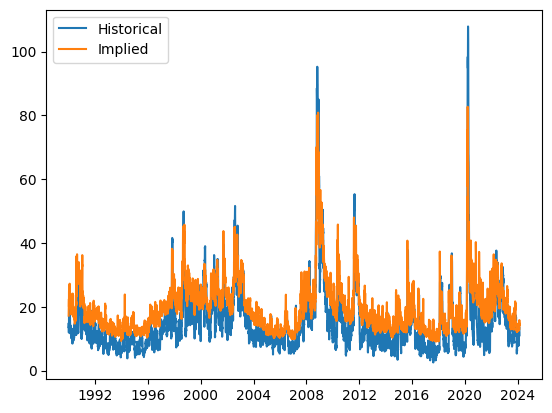
\includegraphics[width=\linewidth]{assets/hist-vs-impl-vol.png}
    \caption{Comparison of historical rolling 1 month volatility and implied 1 month volatility for the S\&P500}
    \label{fig:hist-vs-impl-vol}
\end{figure}

\subsection{Secondary factor model description}
As outlined by \cite{fama_french_1995}, there are other fundamental factors that affect the returns of stocks and of trading strategies. Many of the fundamental factors however, like the Book-to-Market outlined in this paper and others, are only observable as quarterly data in the best case, while all previous factors were observable daily. In order to run the previous factor analysis with as much data density as possible, but also to understand how these other factors affect the strategy's performance, a secondary regression has been created. 

The already presented primary regression is performed on a rolling basis. For every quarter, the primary regression is run and the $\alpha$ of said regression is kept so as to obtain a series of quarterly $\alpha$. These $\alpha$ are then regressed on these new quarterly factors, shedding some light into the drivers of the excess returns found with the first regression. This secondary model is the following.
\begin{multline}
    \label{eq:secondary-regression}
    \alpha^{(1)}=\alpha^{(2)} + \gamma_{MKTVal}MKTVal + \gamma_{BTM}BTM + \gamma_{PER}PER + \gamma_{EVEBIT}EVEBIT + \\ + \gamma_{EVEBITDA}EVEBITDA + \gamma_{GPA}GPA + \gamma_{ROC}ROC + \epsilon^{(2)}
\end{multline}
These factors have been shown to be drivers of portfolio performance in \cite{ramon_bermejo_climent_2021}. The meaning behind those factors is the following
\begin{itemize}
    \item $MKTVal$: The market value of the stock, measured in market capitalization.
    \item $BTM$: The Book-to-Market ratio of the stock.
    \item $PER$: The Price-to-Earnings ratio of the stock.
    \item $EVEBIT$: The Enterprise Value to EBIT ratio of the stock. 
    \item $EVEBITDA$: The Enterprise Value to EBITDA ratio of the stock.
    \item $GPA$: The Gross Profits to Assets ratio of the stock.
    \item $ROC$: The Return on Capital ratio of the stock. 
\end{itemize}
The first 5 regressors are a proxy for the value characteristic of the stock, while the last 2 showcase the profitability characteristic of the stock. 

In a similar way to the last regression, the resampled alpha is regressed in a panel regression over all stocks for all time periods, where each of these factors -- all fundamental -- are unique for each stock. The main difference in how this regression was conducted as oposed to the last one is in the preprocessing of the factors. In this regression, there are some very significant defferences in the order of magnitude of the factors, with some being ratios in the unit scale and others -- namely the Market Value -- being in the order of the billions. In order to avoid numerical problems during the estimation of the coefficients, all factors have been scaled through min-max scaling \cite{amorim_cavalcanti_cruz_2023}.